\documentclass[9pt,pdf,hyperref={unicode}]{beamer}
\beamertemplatenavigationsymbolsempty

\setbeamertemplate{blocks}[rounded=true, shadow=true]
\setbeamertemplate{footline}[page number]
\usepackage{multicol}

\usefonttheme{serif}

\usepackage[utf8]{inputenc}
\usepackage[english, russian]{babel}
\usepackage{amsmath,mathrsfs,mathtext}
\usepackage{graphicx, epsfig}
\usepackage{caption}
\usepackage{subfig}
\usepackage{amsmath, bm}

\usepackage{comment}

\usepackage{tabularx}

\usepackage{tikz}

\DeclareMathOperator*{\argmin}{arg\,min}
\DeclareMathOperator*{\argmax}{arg\,max}

\makeatletter
\let\@@magyar@captionfix\relax
\makeatother

\usetheme{Warsaw}
\usecolortheme{sidebartab}
\definecolor{beamer@blendedblue}{RGB}{31,96,49}

\setbeamertemplate{enumerate items}[circle]

\setbeamersize{text margin left=1.5em, text margin right=1.5em}

\usepackage{ragged2e}

%----------------------------------------------------------------------------------------------------------
\title[\hbox to 56mm{Кластеризация точек временных рядов \hfill\insertframenumber\,/\,\inserttotalframenumber}]
{Анализ свойств локальных моделей в задачах кластеризации точек квазипериодических временных рядов}
\author[Грабовой А.\ В.]{\Large Грабовой Андрей Валериевич}
\institute{ Московский физико-технический институт\\
Факультет управления и прикладной математики\\
Кафедра интеллектуальных систем\\
~\\
Научный руководитель д.ф.-м.н. В.\ В. Стрижов
}

\date{\footnotesize{\emph{Москва}\\
 2019 г}}
%----------------------------------------------------------------------------------------------------------
\begin{document}
%----------------------------------------------------------------------------------------------------------
\begin{frame}
\titlepage
\end{frame}

%----------------------------------------------------------------------------------------------------------
\begin{frame}{Задача кластеризации точек временного ряда}
\justifying
\textbf{Цель:} предложить алгоритм поиска характерных квазипериодических сегментов внутри временного ряда, полученных при помощи мобильного акселерометра.

~\\
\textbf{Задачи}

\begin{enumerate}
\justifying
	\item Предложить признаковое описание точек временного ряда.
	\item Предложить функцию расстояния между точками временного ряда в новом признаковом описании, для их дальнейшей кластеризации.
\end{enumerate}

~\\
\textbf{Исследуемая проблема}
\begin{enumerate}
\justifying
	\item Понижение размерности пространства признаков. Понстроение признакового описания точек временного ряда.
\end{enumerate}

~\\
\textbf{Метод решения}

	Алгоритм поиска характерных сегментов основывается на методе главных компонент для локального снижения размерности сегмента фазовой траектории в окрестности каждой точки временного ряда. Главные компоненты рассматриваются как признаковое описания точек временного ряда.
	
\end{frame}
%----------------------------------------------------------------------------------------------------------
\begin{frame}{Список литературы}
	\begin{enumerate}
	\justifying
		\item \textit{A. P. Motrenko, V. V. Strijov} Extracting fundamental periods to segment biomedical signals~// Journal of Biomedical and Health Informatics, 2015,~20(6). P.~1466--1476.
		\item \textit{A.D. Ignatov, V. V. Strijov} Human activity recognition using quasi-periodic time series collected from a single triaxial accelerometer.~// Multimedia Tools and Applications, 2015, P.~1--14.

		
		\item \textit{Y. G. Cinar and H. Mirisaee} Period-aware content attention RNNs for time series forecasting with missing values~// Neurocomputing,~2018. Vol.~312. P.~177--186.
		
		\item \textit{A. Olivares, J. Ramirez, J. M. Gorris, G. Olivares, M. Damas} Detection of (in)activity periods in human body motion using inertial sensors: A~comparative study.~// Sensors, 12(5):5791--5814,~2012.
		
	\end{enumerate}
\end{frame}

%----------------------------------------------------------------------------------------------------------
\begin{frame}{Постановка задачи кластеризации точек}
\justifying
Сегмент --- последовательность точек временного ряда, которая относится к одному характерному физическому действию человека: шаг, прыжок.\\
Цепь --- последовательность сегментов, которые образуют квазипериодическую последовательность точек.

\begin{center}
	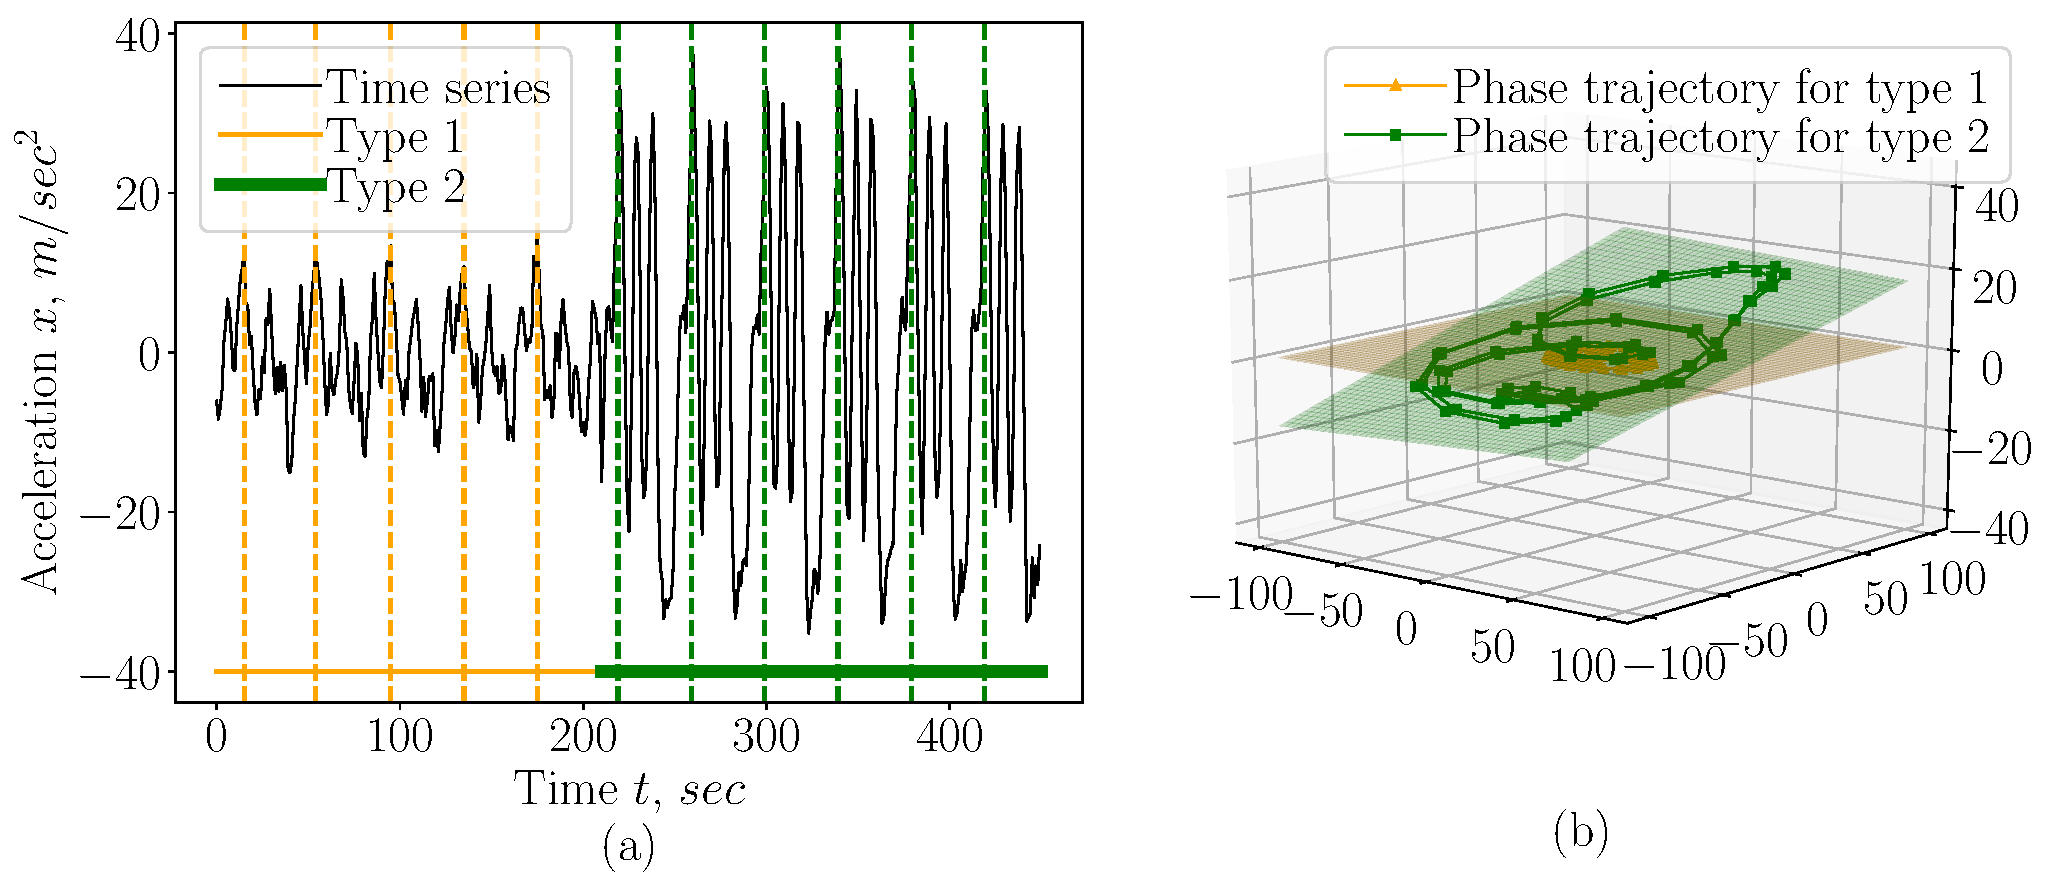
\includegraphics[width=1\textwidth]{results/introduction}
\end{center}

a) временной ряда разбитый на сегменты; b) проекции на плоскость фазовых траекторий временного ряда, которые относятся к Type~1 и Type~2.

\end{frame}

%----------------------------------------------------------------------------------------------------------
\begin{frame}[shrink=5]{Постановка задачи кластеризации точек}
\justifying
Предположения:
\begin{itemize}
	\item число различных типов сегментов внутри временного ряда известно и равно~$K$,
	\item для всех~$\textbf{v} \in \mathcal{V}$ выполняется~$\left|\textbf{v}\right| \leq T$, где~$\left|\textbf{v}\right|$ длина сегмента,
	\item для всех~$i$ либо~$[\textbf{v}_{i-1},\textbf{v}_{i}]$ либо~$[\textbf{v}_{i},\textbf{v}_{i+1}]$  является цепью.
\end{itemize}

Строится отображение
$$
a : t \to \mathbb{Y} = \{1,\cdots, K\}, 
$$
где~$t \in \{1,\cdots, N\}$ некоторый момент времени, на котором задан временной ряд.
Требуется, чтобы отображение~$a$ удовлетворяло следующим свойствам:
$$
\begin{cases}
    a\left(t_1\right) = a\left(t_2\right), &  \text{если в моменты } t_1, t_2 \text{ совершается один тип действий},\\
    a\left(t_1\right) \not= a\left(t_2\right), &  \text{если в моменты } t_1, t_2 \text{ совершаются разные типы действий}.
\end{cases}
$$

~\\
Задана асессорская разметка точек временного ряда:
$$
\textbf{y} \in \{1,\cdots,K\}^{N}.
$$
Ошибка алгоритма~$a$ на временном ряде~$\textbf{x}$:
$$
S = \frac{1}{N}\sum_{t=1}^{N}[y_t = a\left(t\right)],
$$
где~$t$~---~момент времени,~$y_t$ асессорская разметка~$t$-го момента времени для заданого временного ряда.

\end{frame}
%----------------------------------------------------------------------------------------------------------
\begin{frame}[shrink=5]{Построение признакового описания точек}
\justifying

Фазовая траектория ряда $\textbf{x}$:
$$\mathbf{H} = \{\textbf{h}_t| \textbf{h}_t = [x_{t-T}, x_{t-T+1}, \cdots, x_{t}],~T\leq t\leq N\},$$
где $\textbf{h}_t$~---~точка фазовой траектории.

~\\
Множество сегментов фазовой траектории:
$$\mathbf{S} = \{\textbf{s}_t| \textbf{s}_t = [\textbf{h}_{t-T}, \textbf{h}_{t-T+1}, \cdots, \textbf{h}_{t+T-1}],~2T\leq t\leq N-T\},$$
где $\textbf{s}_t$~---~это сегмент фазовой траектории в окрестности момента времени $t$.

\begin{center}
	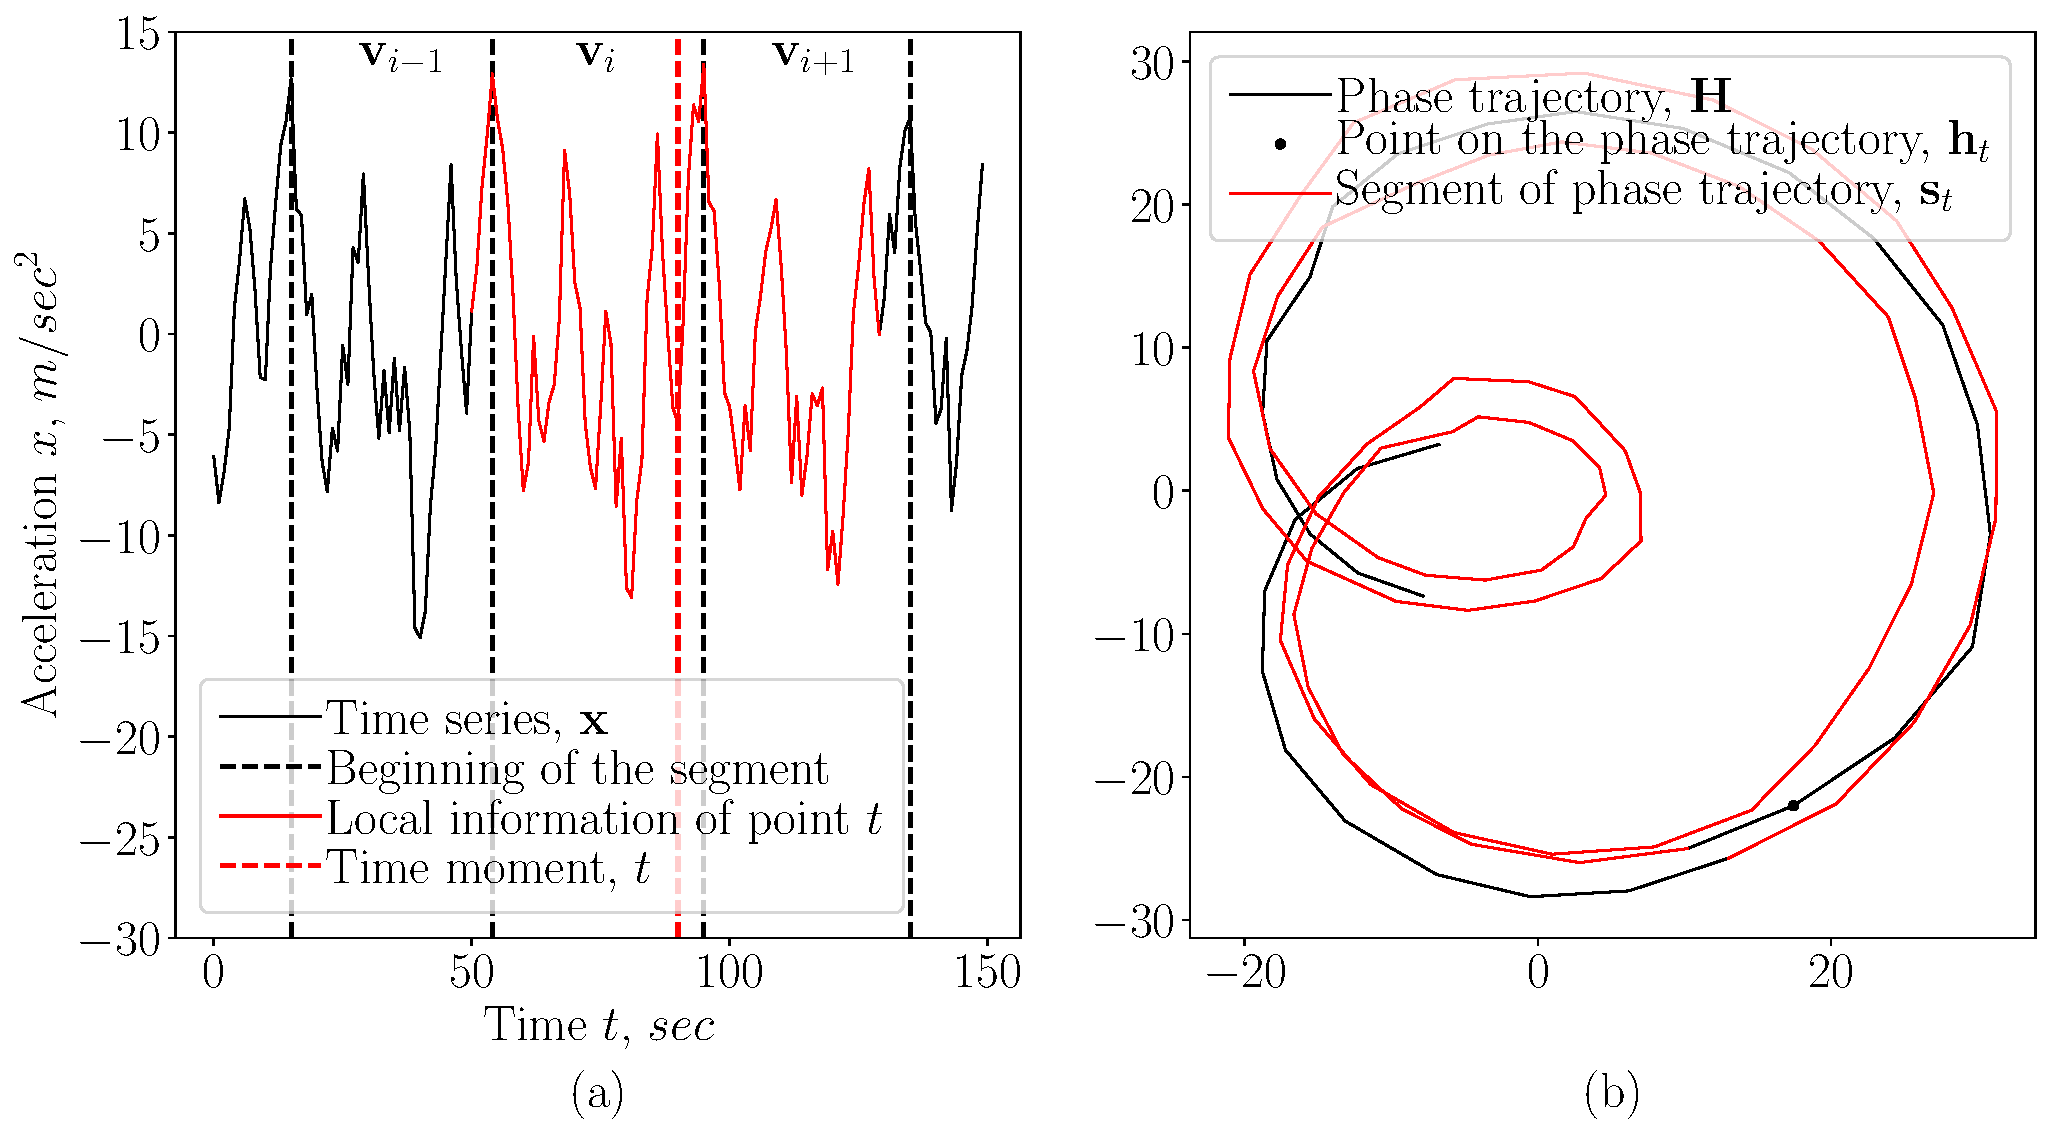
\includegraphics[width=0.8\textwidth]{results/statement}
\end{center}
\end{frame}
%----------------------------------------------------------------------------------------------------------
\begin{frame}{Построение признакового описания точек}
\justifying

Множество базисов, полученных методом главных компонент для каждого сегмента фазовой траектории:
$$\mathbf{W} = \{\textbf{W}_t| \textbf{W}_t = [\textbf{w}^1_t, \textbf{w}^2_t]\}, \quad \bm{\Lambda} = \{\bm{\lambda}_t| \bm{\lambda}_t=[\lambda^1_t, \lambda^2_t]\},$$
где~$[\textbf{w}^1_t, \textbf{w}^2_t]$ и~$[\lambda^1_t, \lambda^2_t]$ это базисные векторы и соответствующие им собственные числа для сегмента фазовой траектории~$\textbf{s}_t$. 

~\\
Далее~$\textbf{W}_t$  и $\bm{\lambda}_t$ рассматриваются как признаковое описанием момента~$t$.

~\\
Для кластеризации точек временного ряда, вводится расстояние в предложенном признаковом описании данного ряда. Расстояние между элементами~$\mathbf{W}_{t_1},\mathbf{W}_{t_2}$:\\
$$\rho\left(\textbf{W}_{t_1}, \textbf{W}_{t_2}\right) = \max\left(\max_{\textbf{e}_2 \in \textbf{W}_{t_2}} d_{1}\left(\textbf{e}_2\right), \max_{\textbf{e}_1 \in \textbf{W}_{t_1}} d_{2}\left(\textbf{e}_1\right)\right),$$
где ~$\textbf{e}_i$ это базисный вектор пространства~$\textbf{W}_i,$ а~$d_i\left(\textbf{e}\right)$ является расстоянием от вектора~$\textbf{e}$ до пространства~$\textbf{W}_i$.

\end{frame}
%----------------------------------------------------------------------------------------------------------

\begin{frame}[shrink=5]{Функция расстояния}
\justifying
Расстояние между элементами~$\mathbf{W}_{t_1},\mathbf{W}_{t_2}$:\\
$$
\rho\left(\textbf{W}_{t_1}, \textbf{W}_{t_2}\right) = \max_{\{\textbf{a},\textbf{b},\textbf{c}\} \subset \textbf{W}_{t_1}\cup \textbf{W}_{t_2} } V\left(\textbf{a},\textbf{b},\textbf{c}\right), 
$$
где~$\textbf{W}_{t_1}\cup\textbf{W}_{t_2}$ это объединение базисных векторов первого и второго пространства,~$V\left(\textbf{a},\textbf{b},\textbf{c}\right)$~---~объем параллелепипеда построенного на векторах~$\textbf{a},$ $\textbf{b},$ $\textbf{c},$ которые являются столбцами матрицы~$\textbf{W}_{t_1}\cup\textbf{W}_{t_2}$.

~\\
Расстояние между собственными числами:\\
$$
\rho\left(\bm{\lambda}_1, \bm{\lambda}_2\right) = \sqrt[]{\left(\bm{\lambda}_1 - \bm{\lambda}_2\right)^{\mathsf{T}}\left(\bm{\lambda}_1 - \bm{\lambda}_2\right)}.
$$

~\\
Расстояние между точками временного ряда:\\
$$
\rho\left(t_1, t_2\right) = \rho\left(\textbf{W}_1, \textbf{W}_2\right) + \rho\left(\bm{\lambda}_1, \bm{\lambda}_2\right).
$$

~\\
Матрица попарных растояний:\\
$$\textbf{M} = \mathbb{R}_{+}^{N\times N}.$$

Используя матрицу попарных расстояний выполняется кластеризация точек временного ряда.
\end{frame}
%----------------------------------------------------------------------------------------------------------
\begin{frame}{Результаты эксперимента}

\begin{itemize}
\justifying
	\item Physical Motion --- ряды получены при помощи мобильного акселерометра.  
	
	Характерные действия: ходьба, бег, приседания.
	\item Synthetic --- синтетические временные ряды.
\end{itemize}

\begin{table}[h!t]
\begin{center}
\label{table:experiment:1}
\begin{tabular}{|c|c|c|c|c|}
\hline
	Ряд,~$\textbf{x}$ &Длина,~$N$& Сегментов,~$K$& Период,~$T$ & Ошибка,~$S$\\
	\hline
	\multicolumn{1}{|l|}{Physical~Motion~1}
	& 900& 2& 50& 0.03\\
	\hline
	\multicolumn{1}{|l|}{Physical~Motion~2}
	& 900& 2& 35& 0.08\\
	\hline
	\multicolumn{1}{|l|}{Physical~Motion~3}
	& 900& 2& 30& 0.09\\
	\hline
	\multicolumn{1}{|l|}{Physical~Motion~4}
	& 800& 2& 50& 0.01\\
	\hline
	\multicolumn{1}{|l|}{Synthetic~1}
	& 2000& 3& 40& 0.008\\
	\hline
	\multicolumn{1}{|l|}{Synthetic~2}
	& 2000& 2& 40& 0.06\\
	\hline
	\multicolumn{1}{|l|}{Synthetic~3}
	& 2000& 2& 40& 0.03\\
	\hline
	\multicolumn{1}{|l|}{Synthetic~4}
	& 2000& 2& 40& 0.03\\
	\hline
	\multicolumn{1}{|l|}{Synthetic~5}
	& 2000& 2& 40& 0.04\\
	\hline
	\multicolumn{1}{|l|}{Simple}
	& 1000& 2& 135& 0.14\\
\hline

\end{tabular}
\end{center}
\end{table}
~\\
\begin{itemize}
	\item $N$ --- число точек во временном ряде,
	\item $K$ --- число различных действий во временном ряде,
	\item $T$ --- максимальная длина сегмента,
	\item $S$ --- точность кластеризации.
\end{itemize}

\end{frame}

%----------------------------------------------------------------------------------------------------------
\begin{frame}{Пример кластеризации точек временного ряда}
\justifying

\begin{center}
	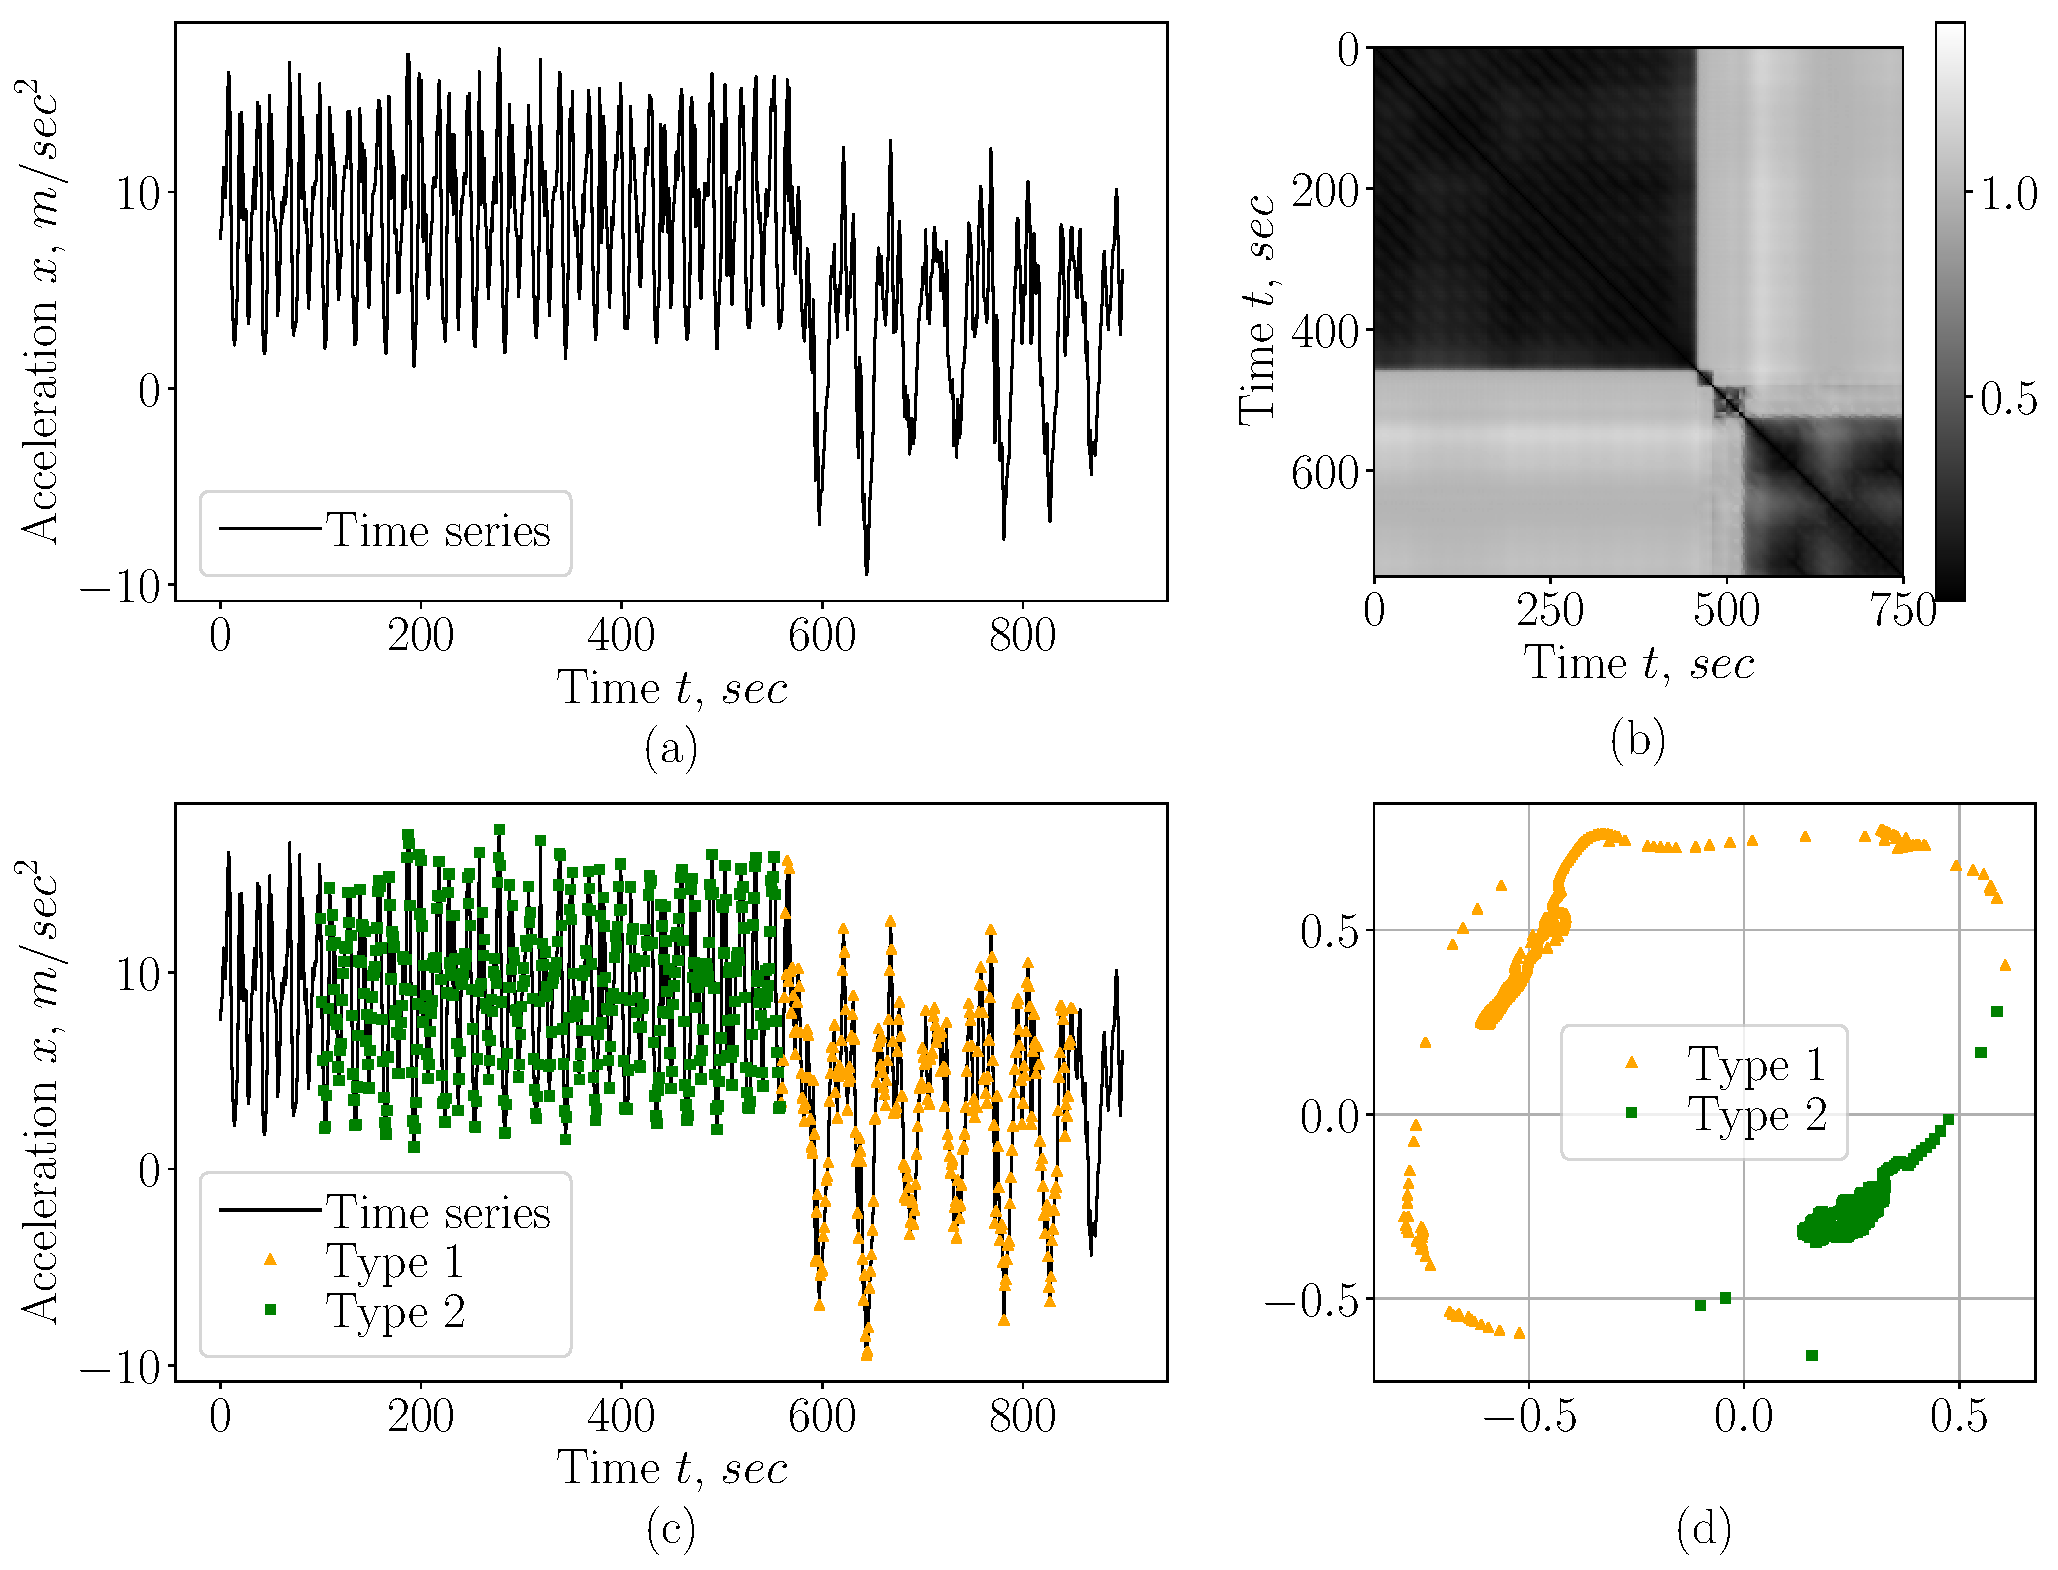
\includegraphics[width=0.8\textwidth]{results/experiment_clustering}
\end{center}

a) начальный временной ряд; b) матрица попарных расстояний; c) кластеризация точек ряда; d) Multidimential Scaling для матрицы попарных расстояний.
\end{frame}
%----------------------------------------------------------------------------------------------------------
\begin{frame}{Пример сегментации временного ряда}
\justifying
\begin{center}
	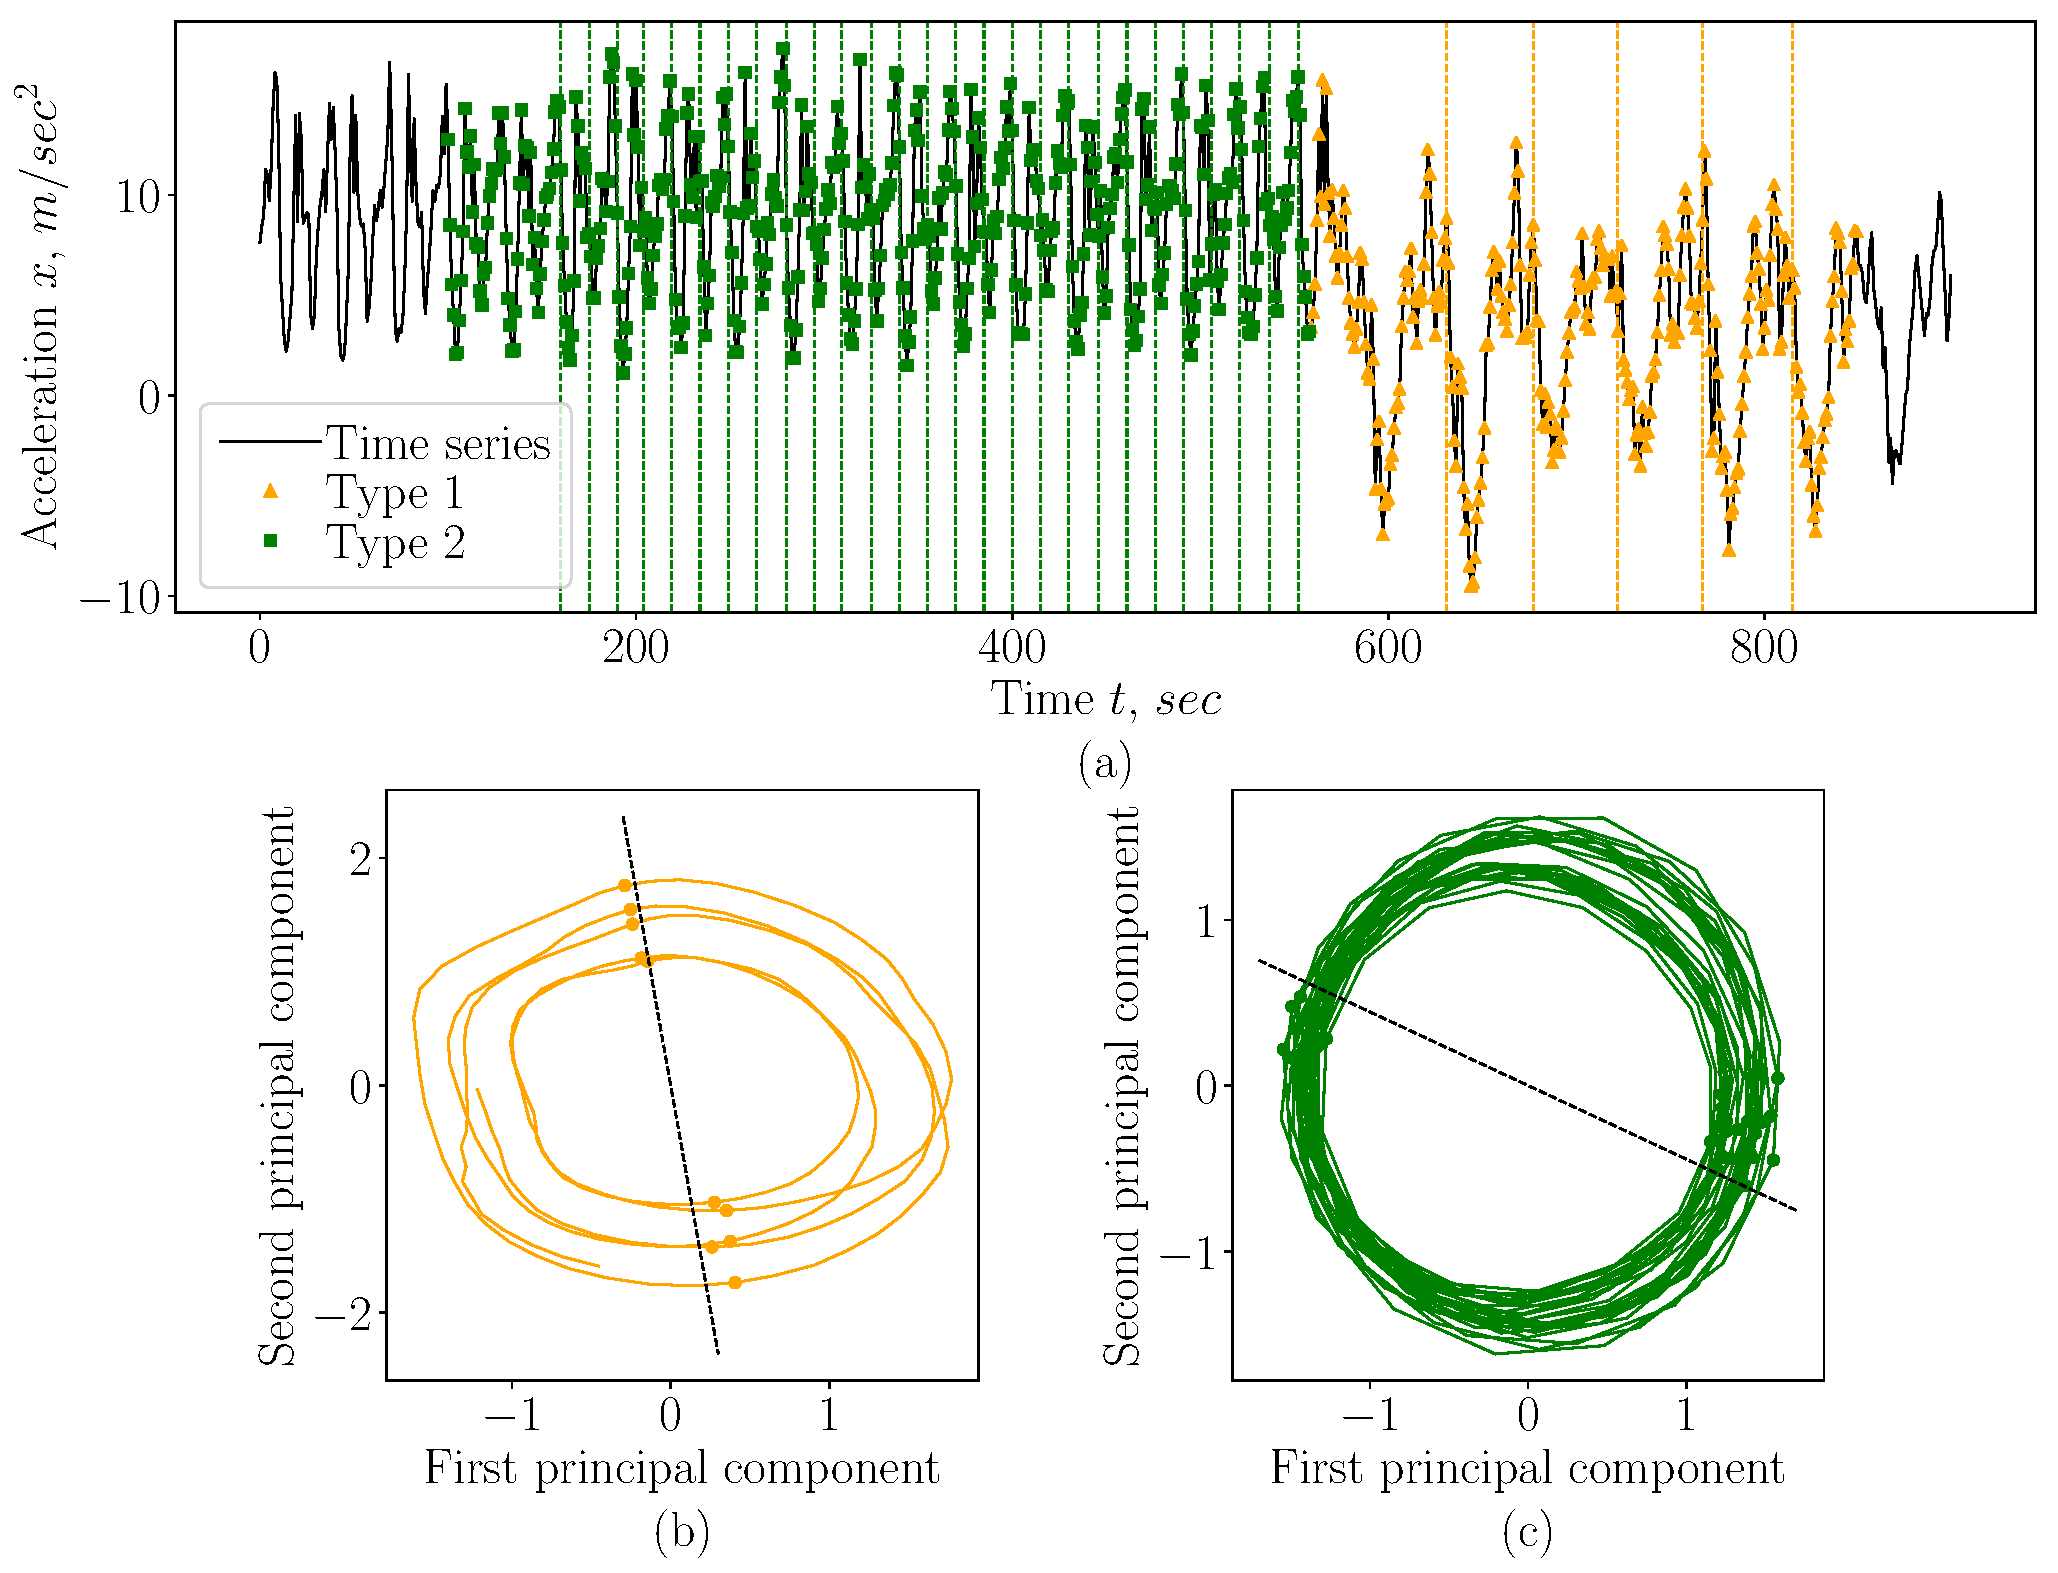
\includegraphics[width=0.8\textwidth]{results/experiment_segmentation}
\end{center}
a) сегментация ряда; b) фазовая траектория для второго действия; c) фазовая траектория для первого действия.

\end{frame}
%----------------------------------------------------------------------------------------------------------

\begin{frame}{Выносится на защиту}
\justifying

	\begin{enumerate}
	\justifying
		\item Предложен алгоритм поиска характерных сегментов, который основывается на методе главных компонент для локального снижения размерности
		\item Введена функция расстояния между локальными базисами в каждый момент времени, которые интерпретировались как признаковое описание точки временного ряда. Данная функция является метрикой.
		\item В ходе эксперимента, на реальных показаниях акселерометра, а также на синтетических данных, было показано, что предложенный метод измерение расстояния между базисами хорошо разделяет точки которые принадлежат различным действиям, что приводит к хорошей кластеризации объектов.
		\item Также в эксперименте была проведена полная сегментация временных рядов для каждого кластера по отдельности.
	\end{enumerate}
	
~\\
~\\
	Планируется решить задачу нахождения минимального размера фазового пространства, для которого  фазовая траектория не имеет самопересечений.
\end{frame}
%----------------------------------------------------------------------------------------------------------
\begin{frame}{Публикации и выступления}
\justifying
	\begin{enumerate}
	\justifying
		\item \textit{Грабовой А. В., Бахтеев О. Ю., Стрижов В. В.} Определение релевантности параметров нейросети // Информатика и ее применения,~2019,~13(2).
		\item \textit{Грабовой А. В., Стрижов В. В.} Анализ свойств локальных моделей в задачах кластеризации квазипериодических временных рядов~// (в~процессе)
		\item \textit{Гадаев Т. Т., Грабовой А. В., Мотренко А. П., Стрижов В. В.} Численные методы оценки объема выборки в задачах регрессии и классификации~// (в~процессе)
		\item \textit{Бучнев Т. Т., Грабовой А. В., Гадаев Т. Т., Стрижов В. В.} Ранее прогнозирование достаточного объема выборки для обобщенно линейной модели~// (в~процессе)
	\end{enumerate}
	
~\\
	\begin{enumerate}
	\justifying
		\item 12 октября 2018. ИОИ-2018. Автоматическое определение релевантности параметров нейросети.
		\item 29 ноября 2019. 61-я Всероссийская научная конференция МФТИ. Поиск оптимальной модели при помощи алгоритмов прореживания.
	\end{enumerate}
	
	
\end{frame}
%----------------------------------------------------------------------------------------------------------

\end{document} 